The \ColorCam{} class extends \Camera{} to represent a color camera. In the \RD{} environment, a color
camera can be a camera sensor connected directly to the computer running the system, or a camera sensor
connected to some other device that sends the images over the network to \RD{}. This versatility is provided 
by \ColorCam{} through the \ColorReceiver{} class. While the color receiver is in charge of acquiring and 
handling the images from the camera, a color camera provides access to the image buffer, the image view, 
and the camera calibration tool. Additionally, it provides the implementation of all abstract methods defined 
by the \Camera{} class. Table \ref{colorcammethods} lists the methods that a color camera adds to the 
base camera representation.

\begin{table}[ht]
\caption{Public methods in the \ColorCam{} class}
\begin{center}
\begin{tabular}{| l |}
	\hline 
	\multicolumn{1}{| c |}{\ColorCam{}} \\
	\multicolumn{1}{| c |}{{\small \texttt{extends} \Camera{}}} \\
	\hline \hline
	\texttt{getImage} \\
	\texttt{getImageView} \\
	\texttt{getCalibrationTool} \\
	\hline
\end{tabular}
\end{center}
\label{colorcammethods}
\end{table}

There are two ways of accessing the camera's images. One way is through the \ColorCam{} object's internal 
image buffer, which stores a copy of the last grabbed image. This image buffer is obtained by calling the
\texttt{get\-Im\-age} method. The second way takes advantage of \RD{}'s intra-application communication 
system and consists of subscribing to the data objects of type \ColorCamData{} through the \DataHandler{} 
interface. The \texttt{han\-dle\-Da\-ta} method of the data handler receives the data objects that contain an 
image buffer with the copy of the grabbed image.

Therefore, every time a call to \texttt{grab\-Im\-age} returns successfully (i.e. returns a \texttt{true} value) two 
things happen: (1) the acquired image is stored in the internal image buffer and (2) it is published through the 
\DataProvider{} interface. Accessing the images from the image buffer gives the user more precision when it
is necessary to process the image right after it is grabbed. Receiving a published image contains the 
overhead of going through the data dispatcher mechanism, but simplifies the communication between
\RD{} applications. 

The \ColorCam{} class adds a second version of the \texttt{grab\-Im\-age} method. This second version takes
as input a value that represents the desired timestamp for the grabbed image. This method is 
useful when synchronizing two or more cameras: given the timestamp of an image from one of the cameras
this \texttt{grab\-Im\-age} method can be used to retrieve the closest corresponding image from the other
cameras.  

A color camera also provides the option of displaying the image stream using \RD{}'s graphics display system.
This is achieved by instantiating an \ImageView{} object linked to the color camera's internal image buffer. 
Every time an image is acquired the image view needs to be refreshed in order to display the new data on the 
buffer. This image view is accessed by calling the \texttt{get\-Im\-age\-View} method.

Finally, the methods to perform camera calibration and retrieve the camera's parameters are available 
through the \CalibrationTool{} object that is associated with every instance of \ColorCam{}. Upon the creation
of the color camera, a calibration tool object is constructed and linked to the camera's internal image buffer. 
When the \texttt{start\-Cal\-i\-bra\-tion} method is called, the calibration tool is started. Then, the user can
use the methods in the calibration tool, obtained by calling the \texttt{get\-Cal\-i\-bra\-tion\-Tool} method, to 
calibrate the camera (see Section \ref{calibrationtool}). 

The following sections present and discuss the modules that compose the \ColorCam{} class. The 
module dependency diagram in Figure \ref{colorcammoduledependency} shows how these classes 
are related to each other. 

\begin{figure}[t]
\begin{center}
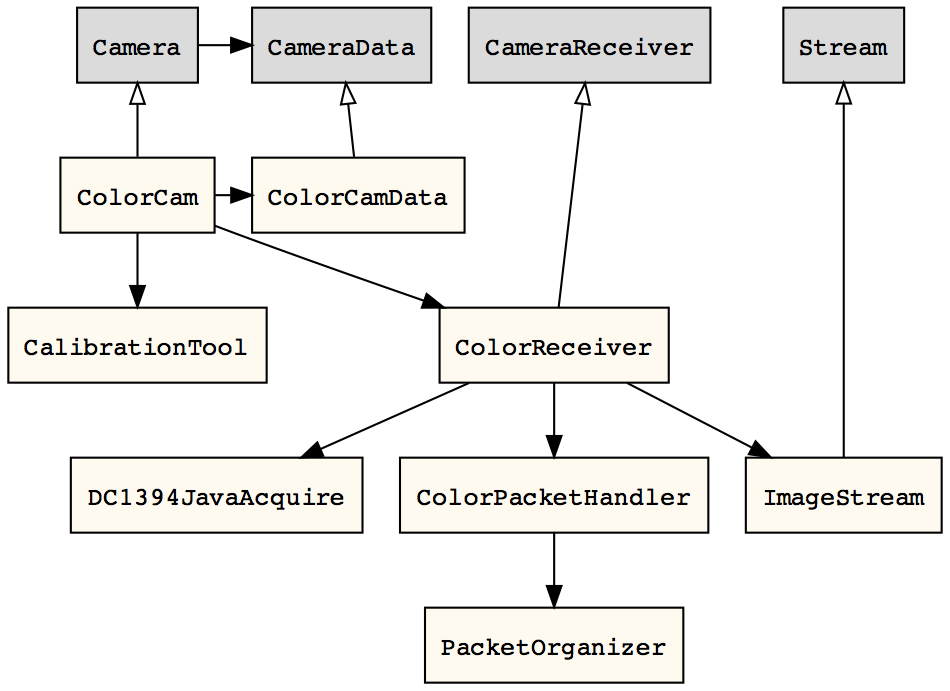
\includegraphics[width = 15cm]{ColorCam.png}
%\digraph[scale=0.75]{ColorCam}{
	graph [rankdir = "TB" margin = 0];
	node [shape = "box" style = "filled" fillcolor = "gainsboro" fontsize = "12" fontname = "Courier"];
		Camera CameraReceiver CameraData Stream;
	node [shape = "box" style = "filled" fillcolor = "floralwhite" fontsize = "12" fontname = "Courier"];
	{ rank = "source"; CameraReceiver Camera CameraData Stream;}
	{ rank = "same"; ColorCam ColorCamData;}
	{ rank = "same"; ColorReceiver CalibrationTool;}
	{ rank = "same"; ColorPacketHandler DC1394JavaAcquire ImageStream;}
	{ rank = "sink"; PacketOrganizer;}
	edge [arrowhead = "normal"];
	Camera -> CameraData;
	ColorCam -> Camera [arrowhead = "empty"] ;
	ColorCam -> ColorCamData;
	ColorCam -> ColorReceiver ;
	ColorCam -> CalibrationTool;
	ColorCamData -> CameraData [arrowhead = "empty"];
	ColorReceiver -> CameraReceiver [arrowhead = "empty"];
	ColorReceiver -> ColorPacketHandler;
	ColorReceiver -> DC1394JavaAcquire;
	ColorReceiver -> ImageStream;
	ImageStream -> Stream [arrowhead = "empty"];
	ColorPacketHandler -> PacketOrganizer;
}
\caption[\ColorCam{}'s module dependency diagram]{\ColorCam{} module dependency diagram. Arcs with 
white arrows represent subtype relations (A $\vartriangleright$ B = A extends B) while arcs with black arrows 
represent implementation relations (A $\blacktriangleright$ B = A uses B). Gray rectangles represent abstract 
classes. The \ImageBuffer{} class is omitted from this diagram.}
\label{colorcammoduledependency}
\end{center}
\end{figure}


